\documentclass[12pt,journal,compsoc,onecolumn]{IEEEtran}
\usepackage{graphicx}
\usepackage{cite}
\usepackage{url}
\usepackage{caption}

\providecommand{\PSforPDF}[1]{#1}
\newcommand{\um} {$\mu$m}
\newcommand{\uW} {$\mu$W}

\newcommand\MYhyperrefoptions{bookmarks=true,bookmarksnumbered=true,
pdfpagemode={UseOutlines},plainpages=false,pdfpagelabels=true,
colorlinks=true,linkcolor={black},citecolor={black},pagecolor={black},
urlcolor={black},
pdftitle={Third interim report},%<!CHANGE!
pdfsubject={Typesetting},%<!CHANGE!
pdfauthor={Carsten Bruns \& Jakob Toft},%<!CHANGE!
pdfkeywords={High-speed communication, Voltage-mode driver, Low-power 10GB/s}}%<^!CHANGE!

% correct bad hyphenation here
\hyphenation{op-tical net-works semi-conduc-tor}

\usepackage[]{units}
\usepackage{graphicx}
\usepackage{subfigure}

\usepackage{epstopdf}

\usepackage{pgfplots} 
\usepgfplotslibrary{external}
\tikzexternalize

\usepackage{float}

\begin{document}
%
% paper title
% can use linebreaks \\ within to get better formatting as desired
\title{Design, Analysis and Simulation of an I/O Link\\Second interim report}

\author{Carsten Bruns
        \& Jakob Toft% <-this % stops a space

%\IEEEcompsoctitleabstractindextext{%
%\begin{abstract}
%\boldmath
%The abstract goes here.
%\end{abstract}


% Note that keywords are not normally used for peerreview papers.
\begin{IEEEkeywords}
High-Speed Data Links, Low-Power 10Gb/s link.
\end{IEEEkeywords}}


% make the title area
\maketitle

\IEEEdisplaynotcompsoctitleabstractindextext
\IEEEpeerreviewmaketitle

<<<<<<< HEAD

=======
>>>>>>> 3debf833a094be1a2bf5601a201b3bc4a838fbe5
\section{Choice of the citcuit topology}

\IEEEPARstart{T}{odo} write sth here! \cite{cressler2007a}
\section{Transmitter schematics}

%TODO explain layering
%TODO explain sizing!! and give the values!

\begin{figure}[ht]
  \centering
  {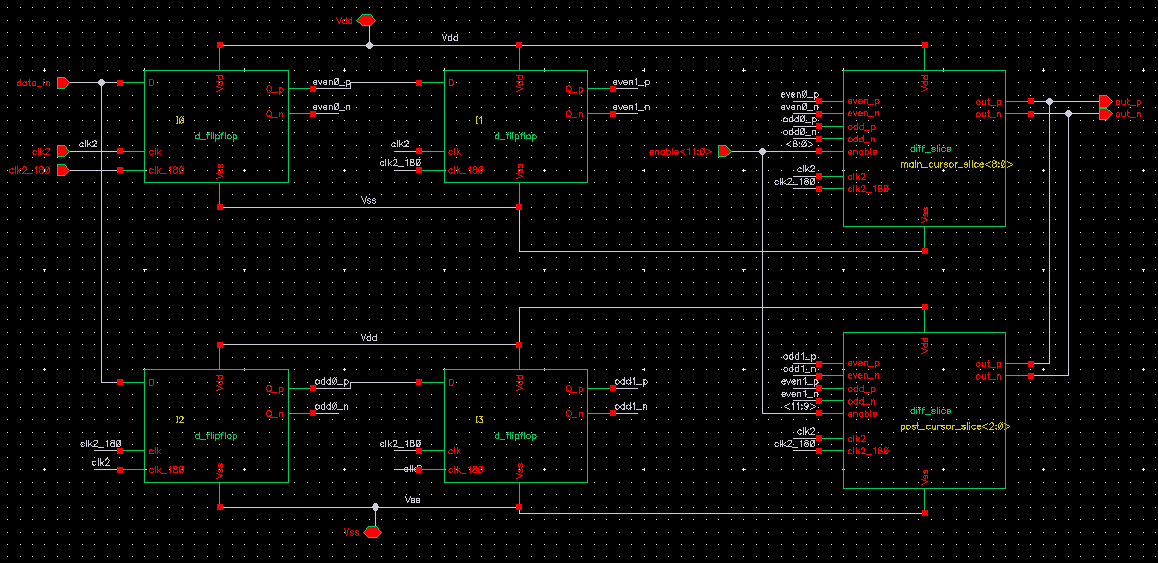
\includegraphics[scale=0.55]{img/transmitter.png}}
  \caption{Transmitter top level circuit}
  \label{fig:top_level}
\end{figure}

\begin{figure}[ht]
  \centering
  \subfigure[Differential slice]
  {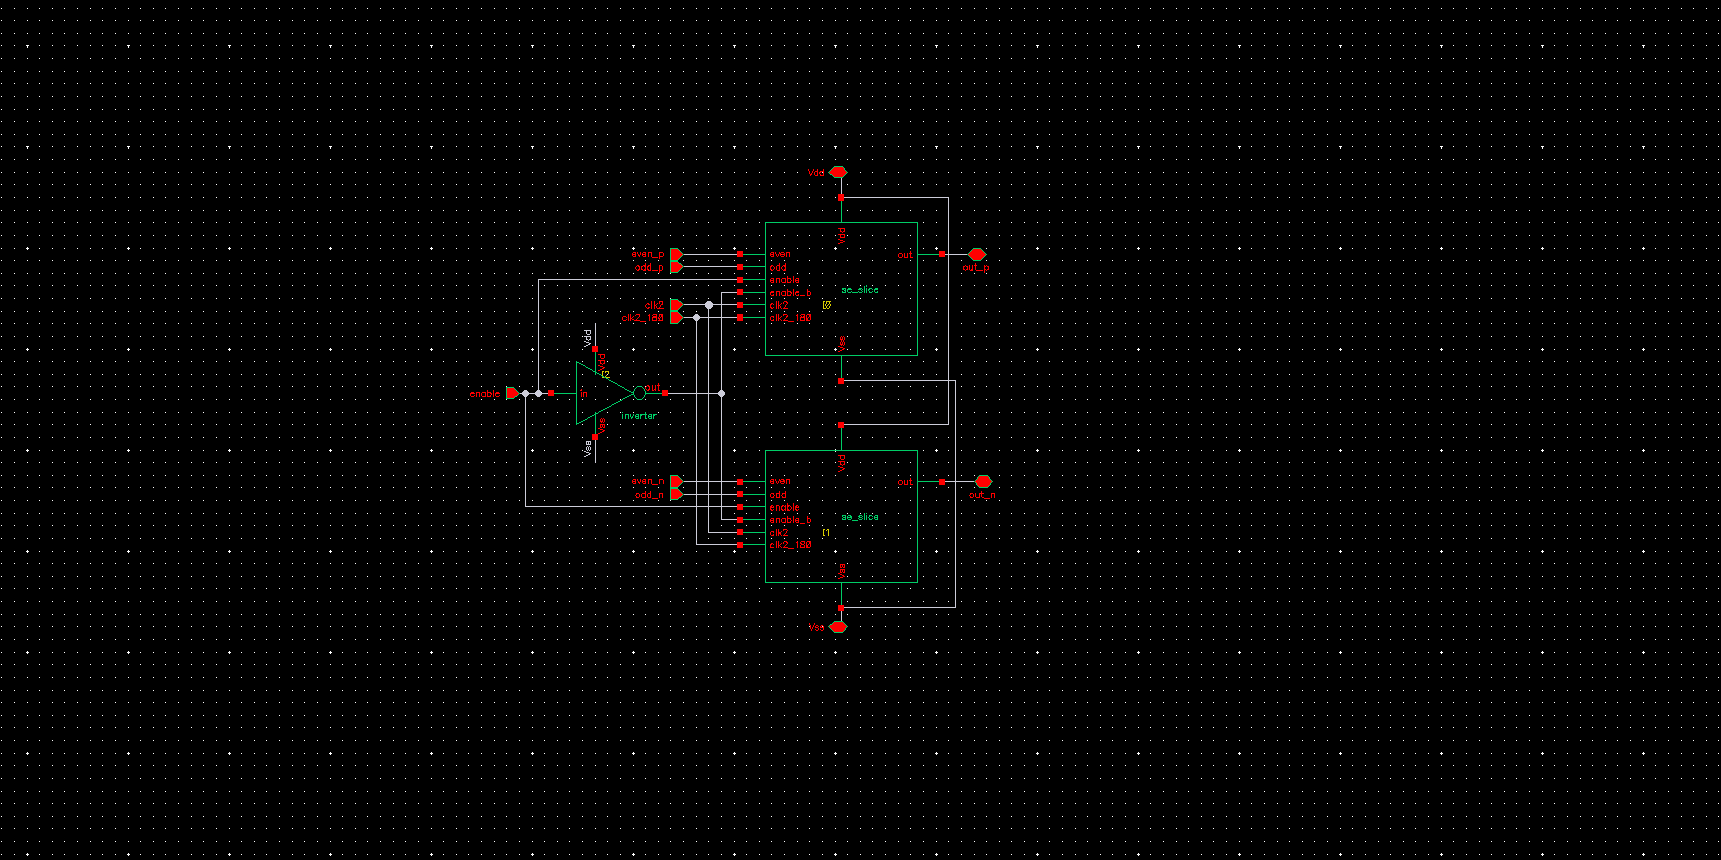
\includegraphics[scale=0.6]{img/diff_slice.png}}
  \subfigure[Single-ended slice]
  {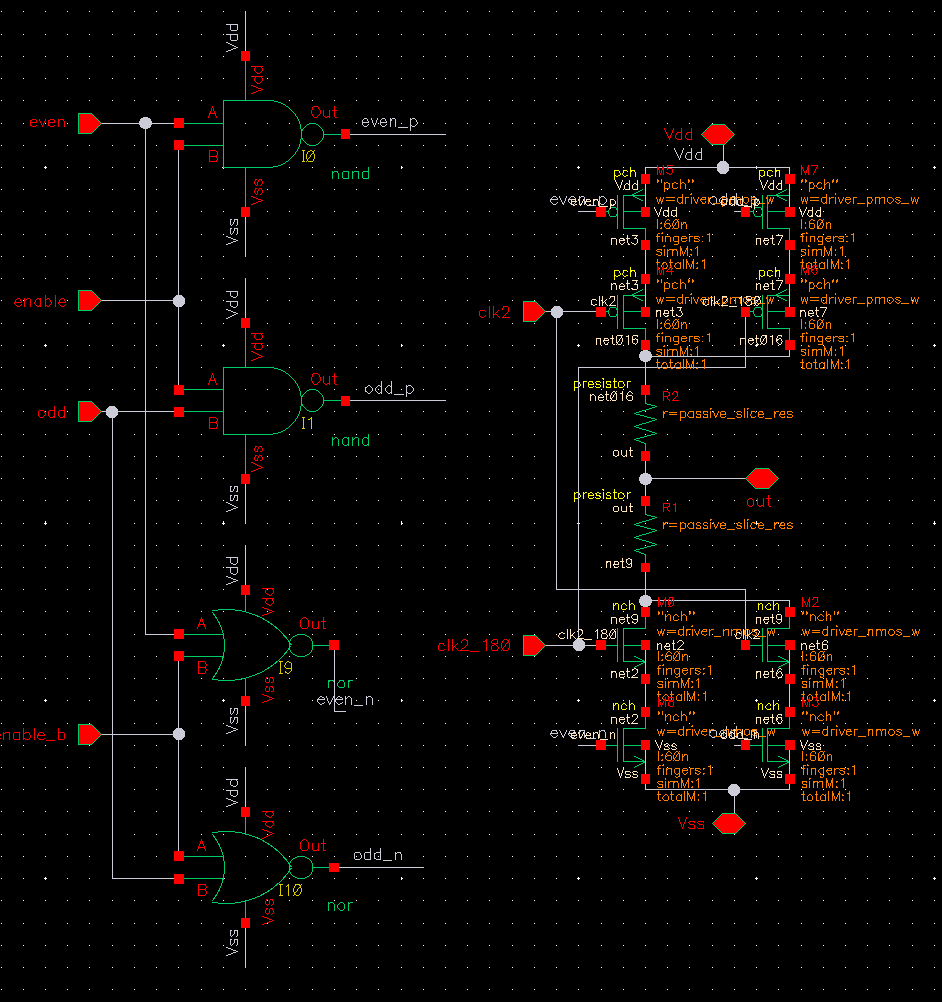
\includegraphics[scale=0.5]{img/se_slice.png}}
  \caption{Slice circuits}
  \label{fig:slices}
\end{figure}

\begin{figure}[ht]
  \centering
  {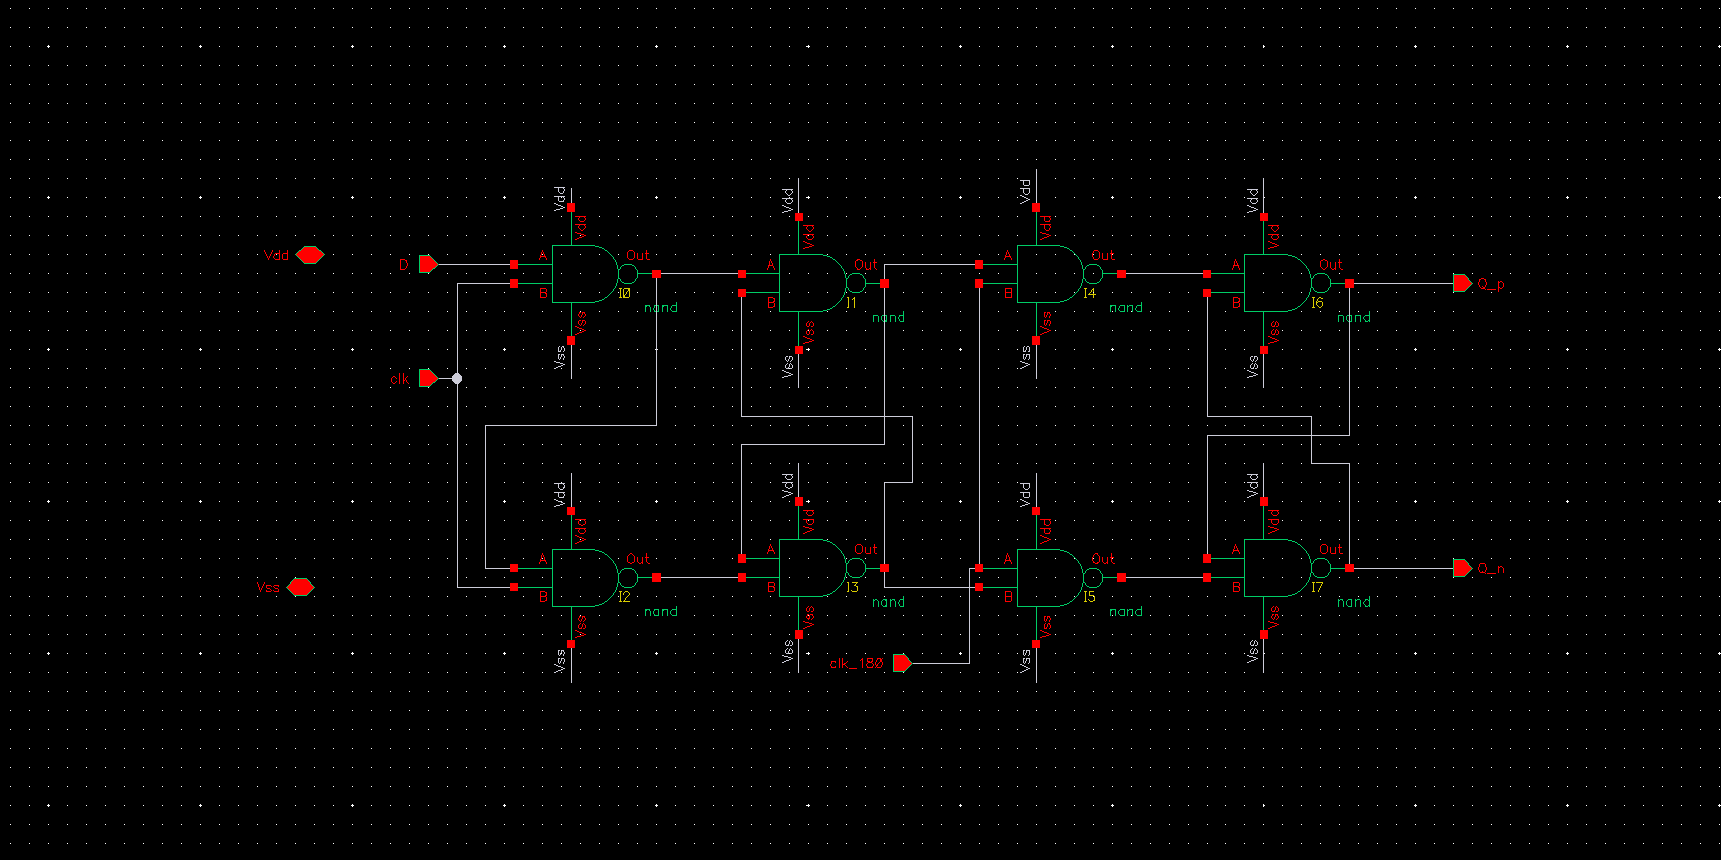
\includegraphics[scale=0.47]{img/flipflop.png}}
  \caption{D-Flipflop}
  \label{fig:flipflop}
\end{figure}

\begin{figure}[ht]
  \centering
  \subfigure[Inverter]
  {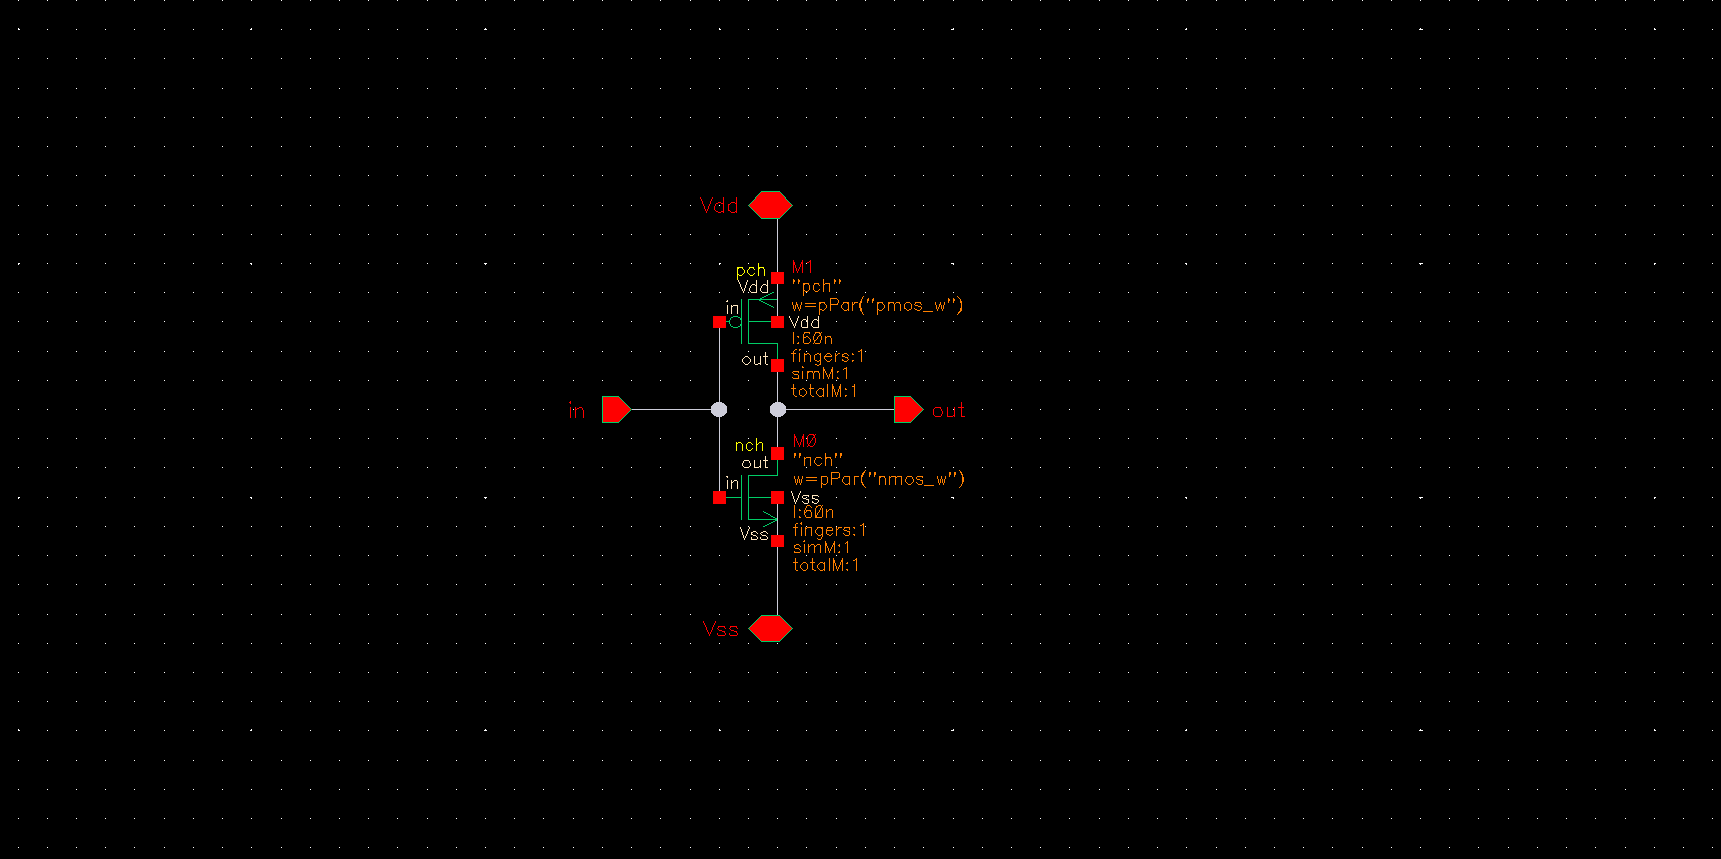
\includegraphics[scale=0.5]{img/inverter.png}}
  \subfigure[NAND gate]
  {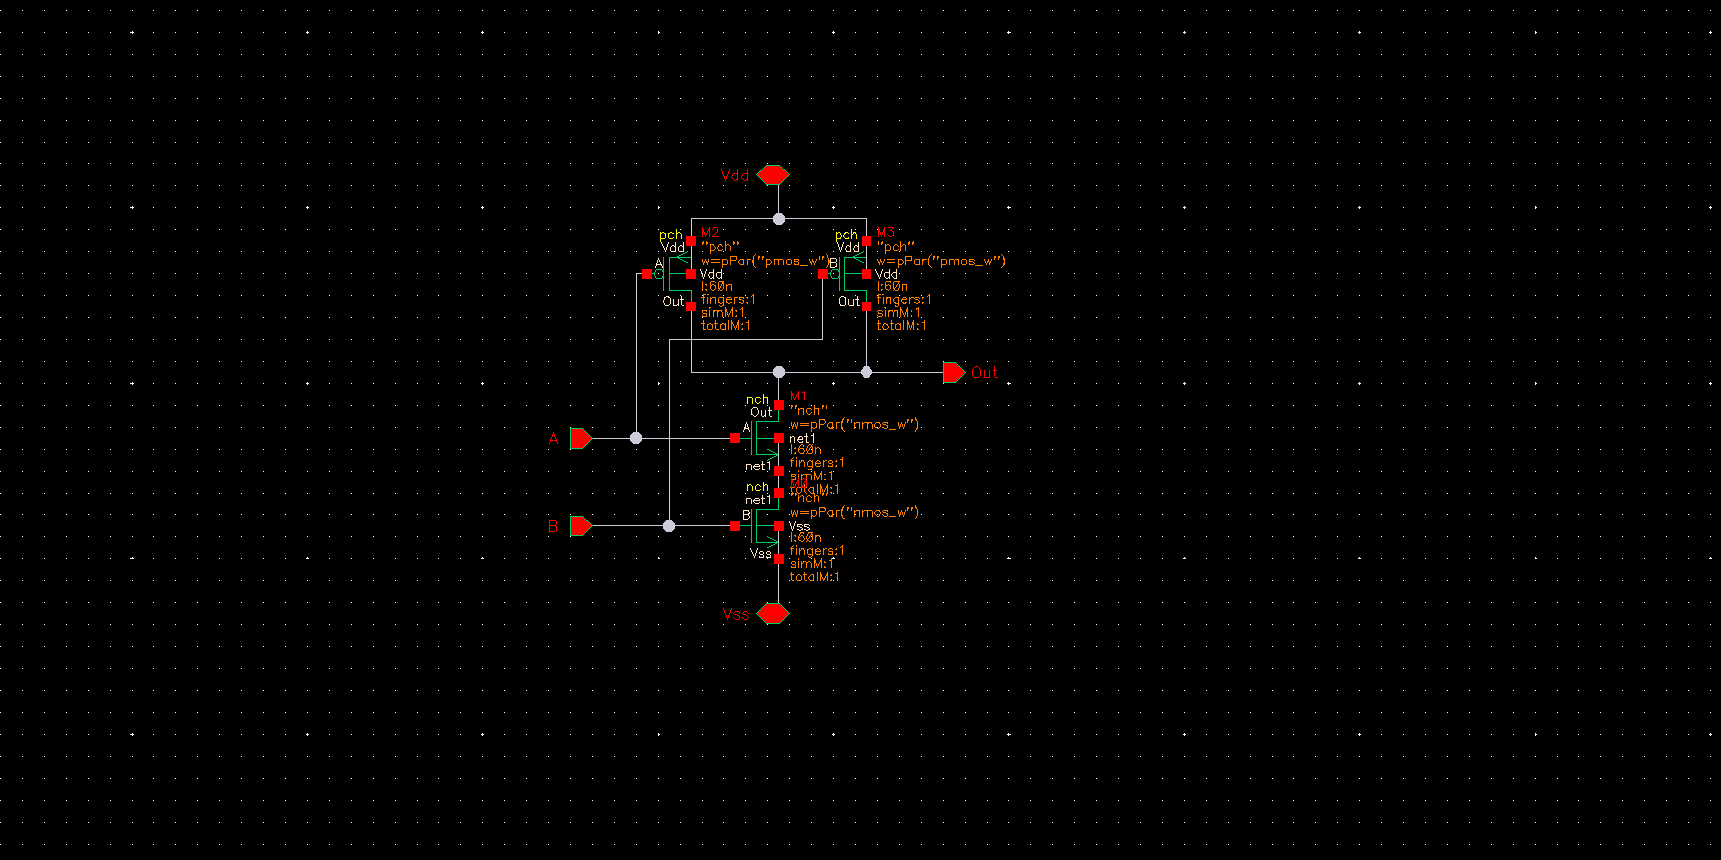
\includegraphics[scale=0.5]{img/nand.png}}
  \subfigure[NOR gate]
  {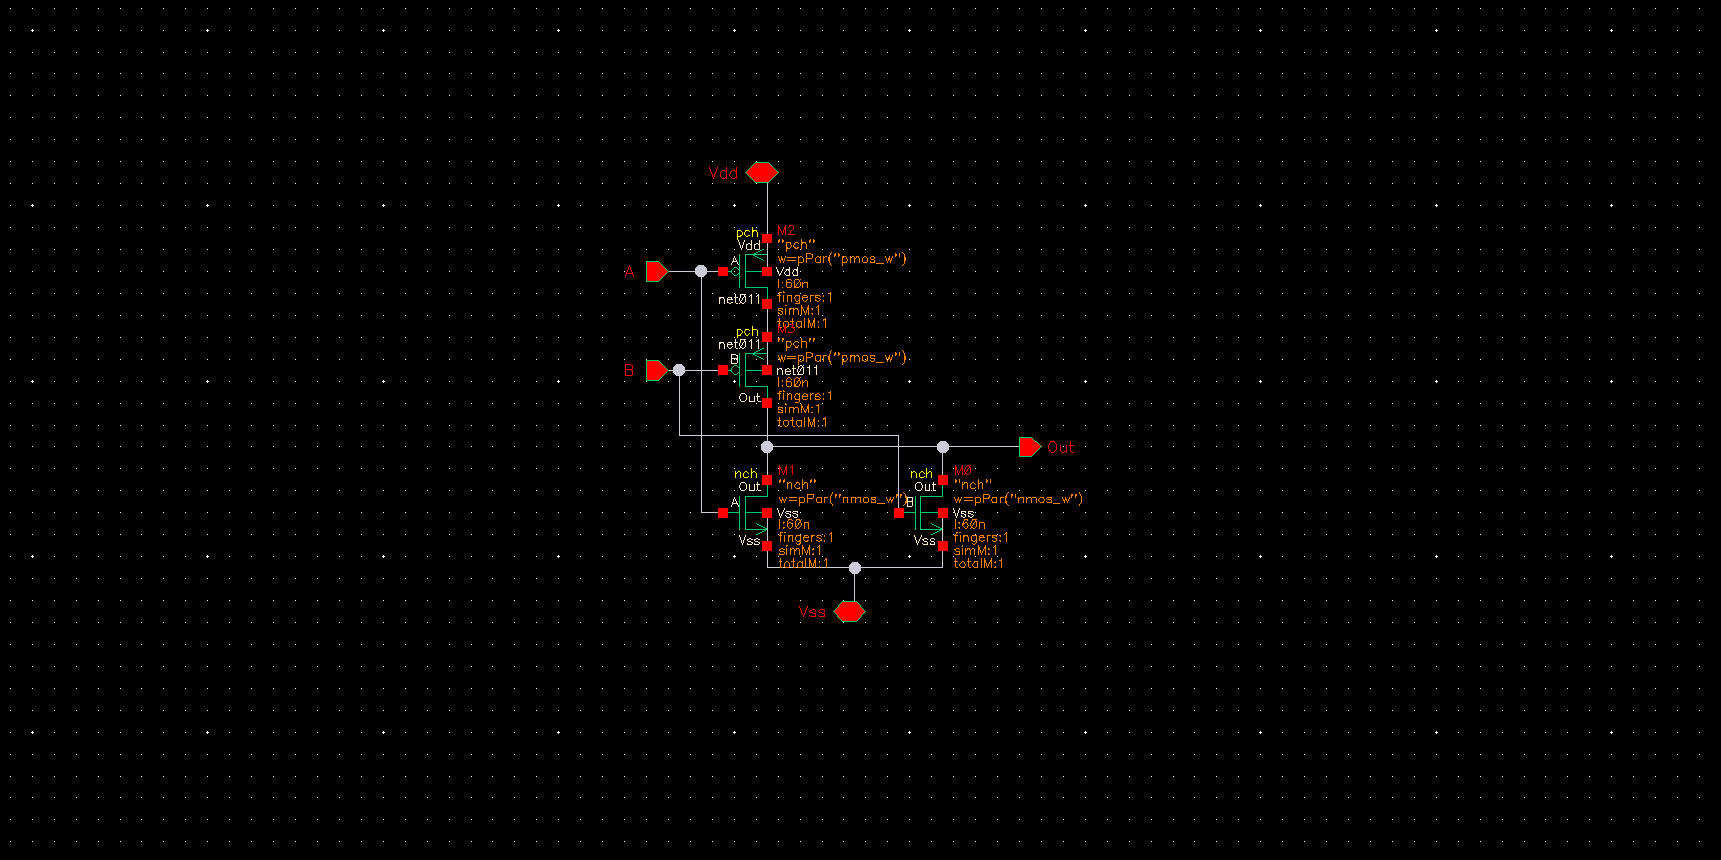
\includegraphics[scale=0.5]{img/nor.png}}
  \caption{Simple gate circuits}
  \label{fig:gates}
\end{figure}
\subsection{Simulations}
\label{sec:simulations}
Figure \ref{fig:strongARM_out} shows the output of the stongARM latch for alternating data at the input for \unit[6]{UI}. For the simulation a data pattern of 11001100 was feed into the input of the receiver. As we have two slices with half-rate clocking this results in alternating data for one of the slices. To degenerate the signal and take the limited bandwith of the channel into account a RC circuit was used at the receiver input resulting in the \textit{in+} and \textit{in-} signals. The \textit{set} and \textit{reset} signals are the direct outputs of the strongARM circuit and the \textit{RS\_out} signal is one of the RS-FlipFlop outputs.

The frequency response of the variable offset amplifier (VOA) is shown in figure \ref{fig:voa_freq} and its ac noise response is drawn in figure \ref{fig:voa_noise}.

\begin{figure}[H]
  \centering
  {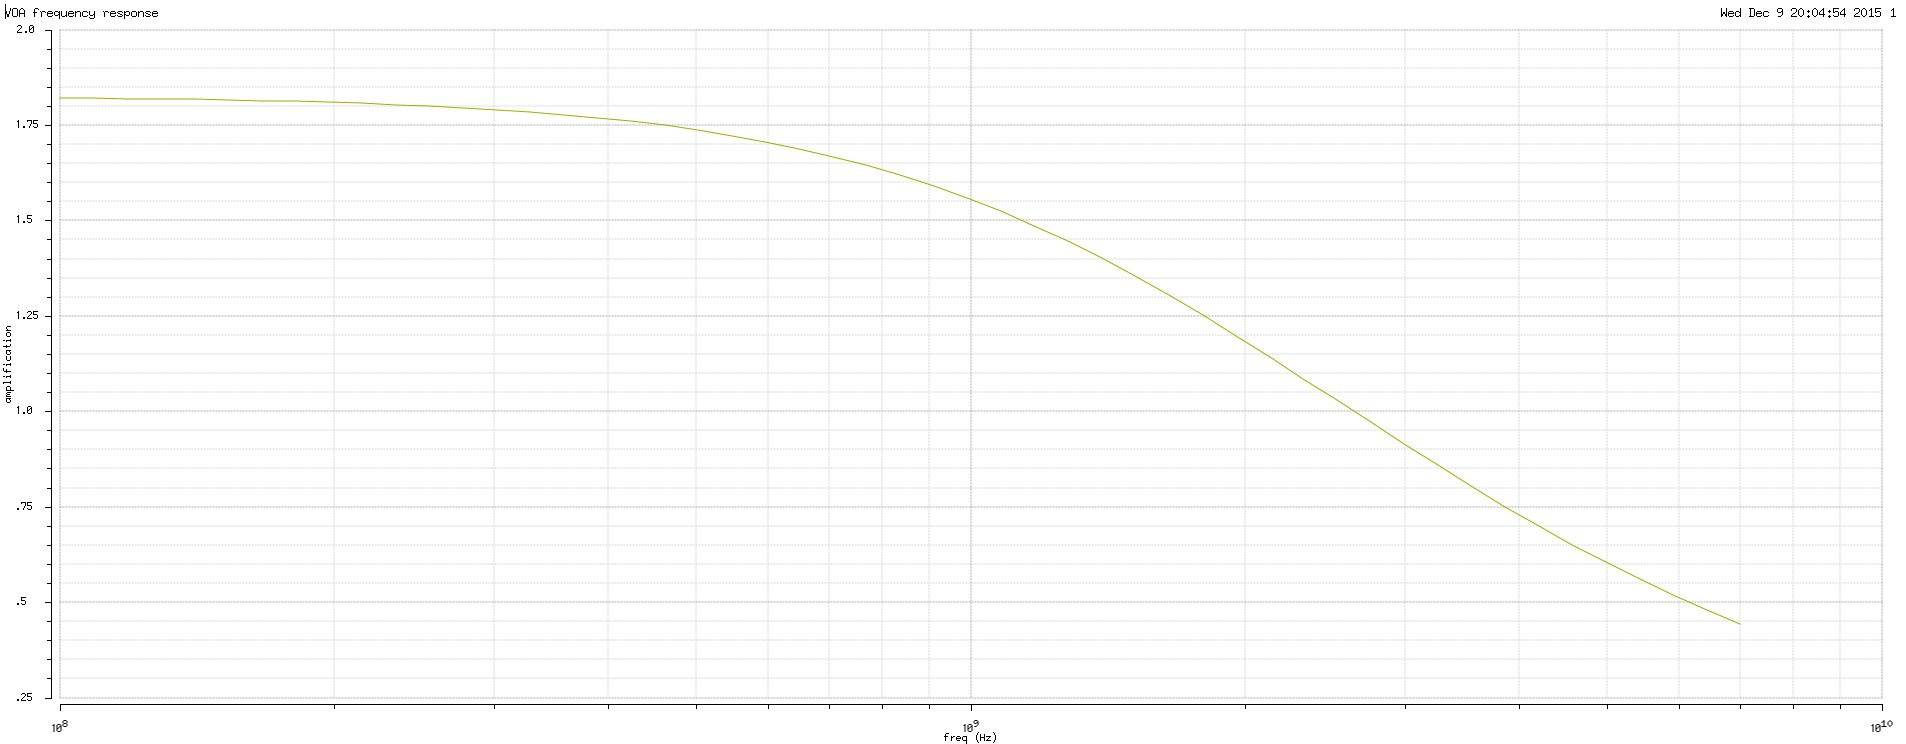
\includegraphics[scale=0.35]{img/voa_freq.jpg}}
  \caption{VOA frequency response}
  \label{fig:voa_freq}
\end{figure}

\begin{figure}[H]
  \centering
  {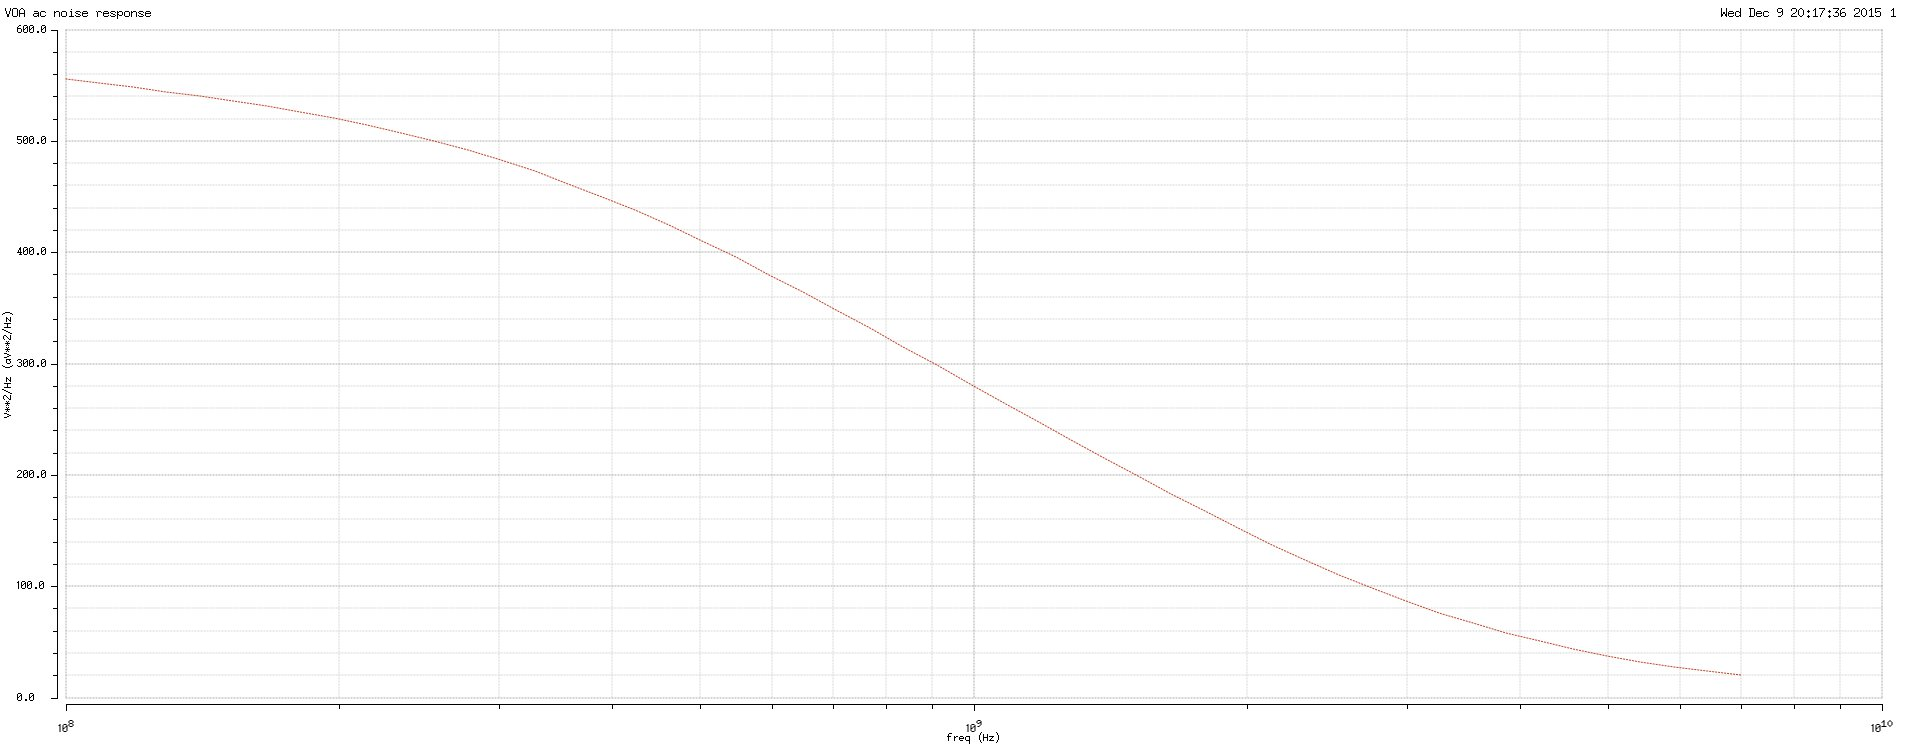
\includegraphics[scale=0.35]{img/voa_noise.jpg}}
  \caption{VOA ac noise response}
  \label{fig:voa_noise}
\end{figure}

\begin{figure}[H]
  \centering
  {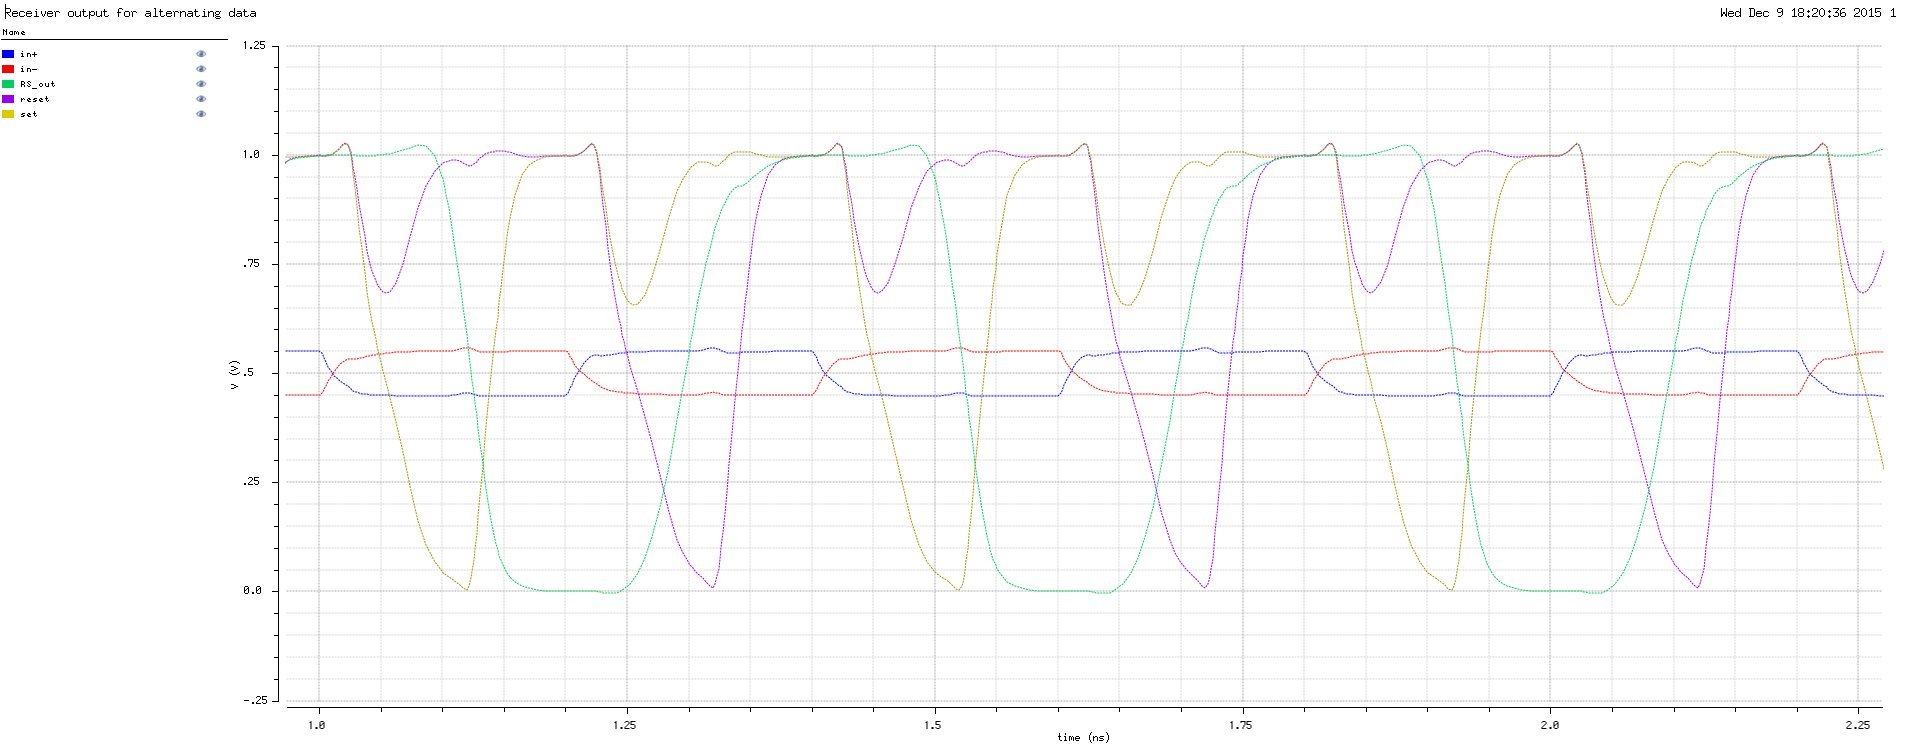
\includegraphics[angle=90, scale=0.47]{img/output_alt_trans.jpg}}
  \caption{Transient waveform for alternating data at the output of the strongARM latch}
  \label{fig:strongARM_out}
\end{figure}

In figure \ref{fig:rx_slice_pdf_cdf} the CDF and PDF for a single receiver slice are shown. As hysteresis was greater than the noise (resulting in a step function as CDF) the simulation was done with scaling transient noise by a factor of four. Therefore to get the right values for the noise the x-axis has to be divided by 4.

\begin{figure}[H]
  \centering
  \subfigure[CDF]
  {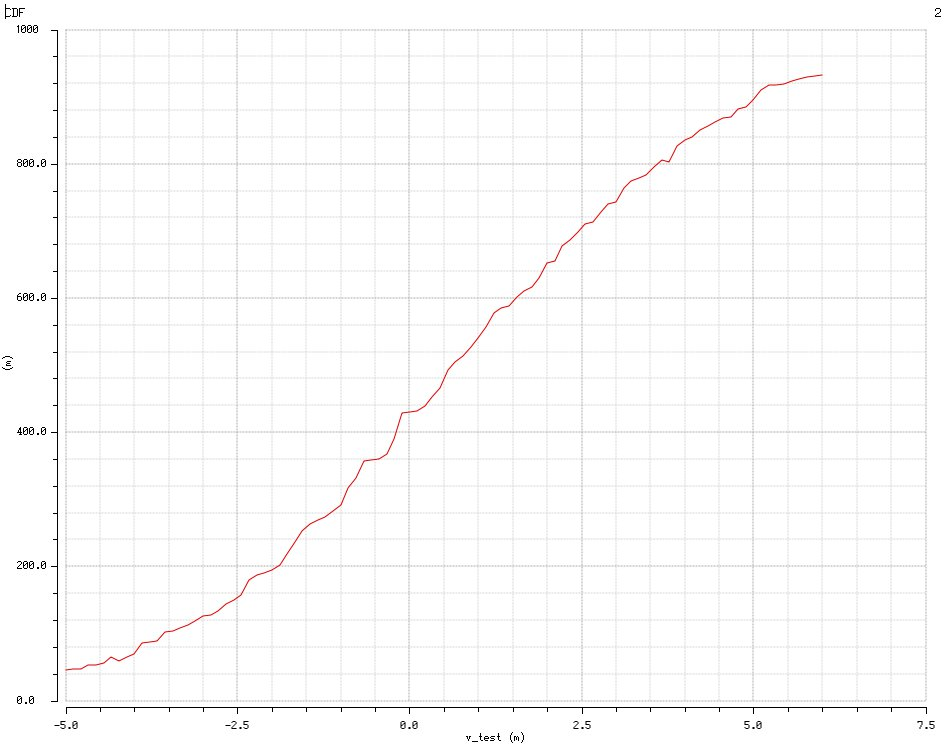
\includegraphics[scale=0.5]{img/rx_slice_cdf.jpg}}
  \subfigure[PDF - logarithmic scale]
  {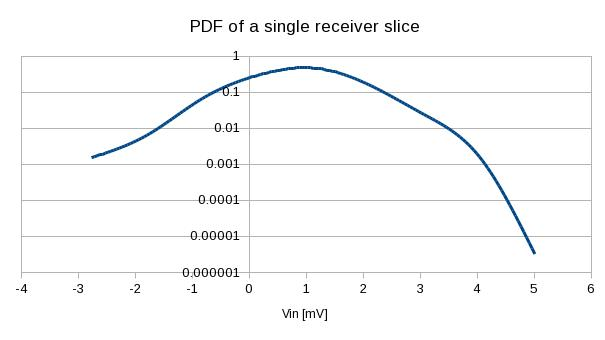
\includegraphics[scale=0.4]{img/rx_slice_pdf.jpg}}
  \subfigure[PDF - linear scale]
  {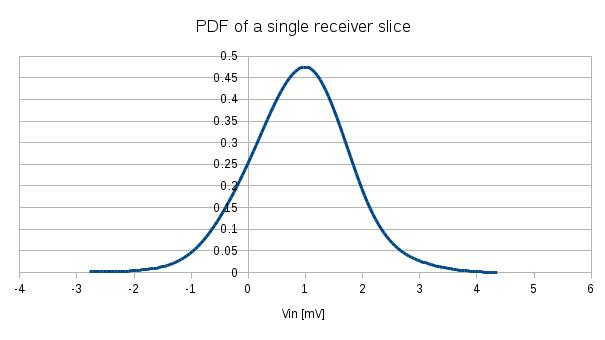
\includegraphics[scale=0.4]{img/rx_slice_pdf_lin.jpg}}
  \caption{Input referred transient noise for a single RX slice}
  \label{fig:rx_slice_pdf_cdf}
\end{figure}

Figure \ref{fig:rx_inp_wc_eye} shows the eye diagram at the reciever input for the worst-case data pattern.

\begin{figure}[H]
  \centering
  {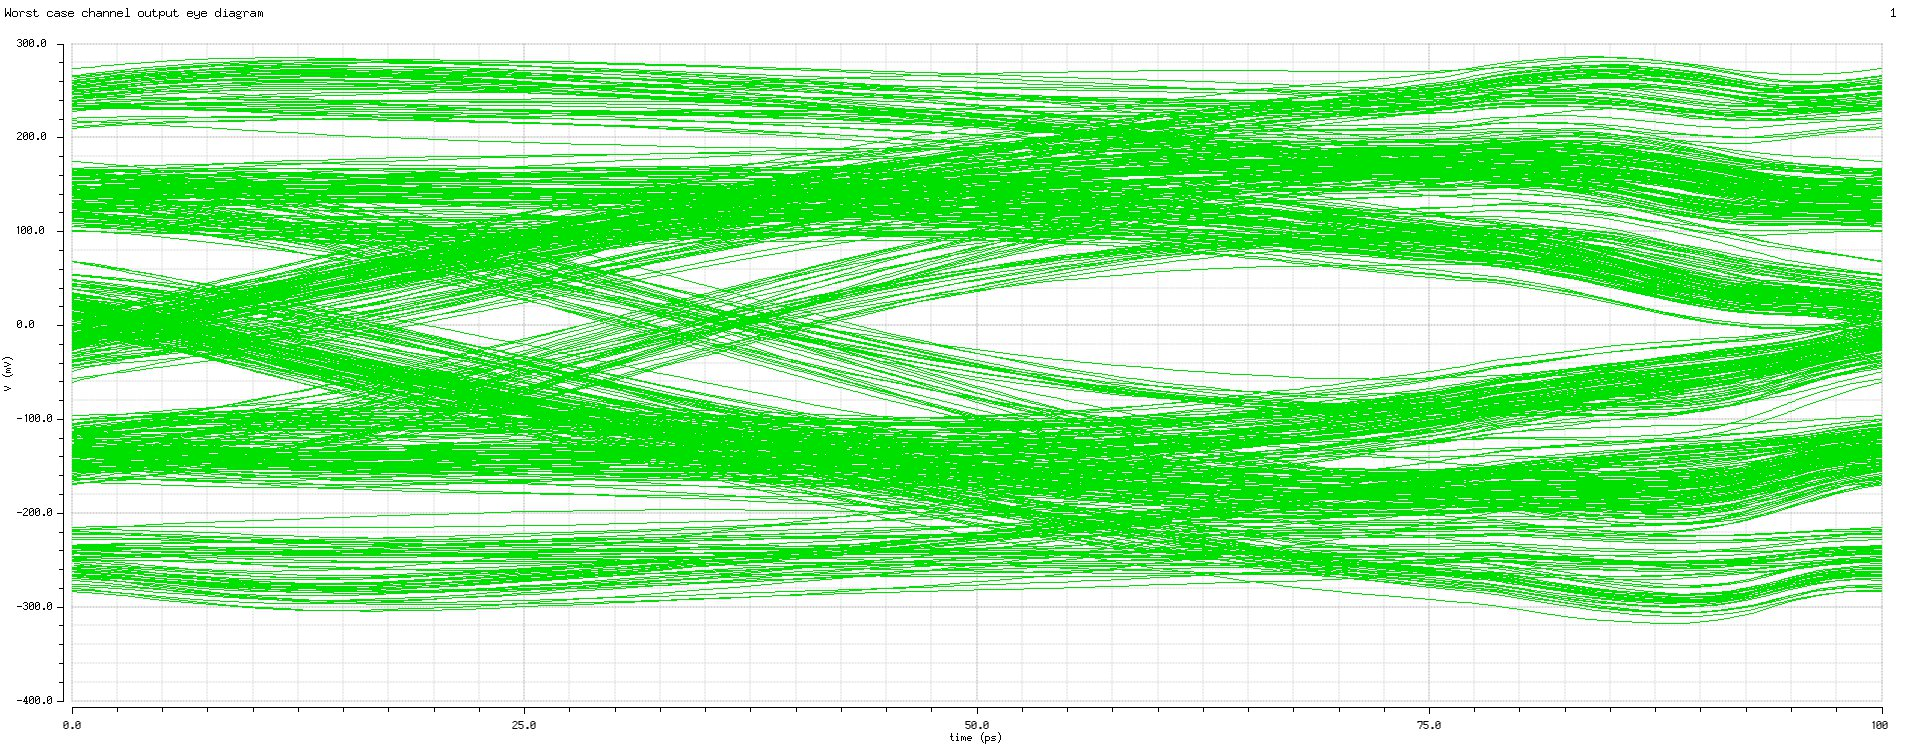
\includegraphics[scale=0.33]{img/wc_ch_eye.jpg}}
  \caption{Eye diagram at the receiver input for worst-case data pattern}
  \label{fig:rx_inp_wc_eye}
\end{figure}


The eye diagram for \unit[5000]{UI} at the receiver input is given in figure \ref{fig:rx_out_eye}. We did not simulate for \unit[10000]{UI} for the same reason as for the transmitter, our limited quota.

\begin{figure}[H]
  \centering
  {subfigure[10Gb/s at 1V]
  {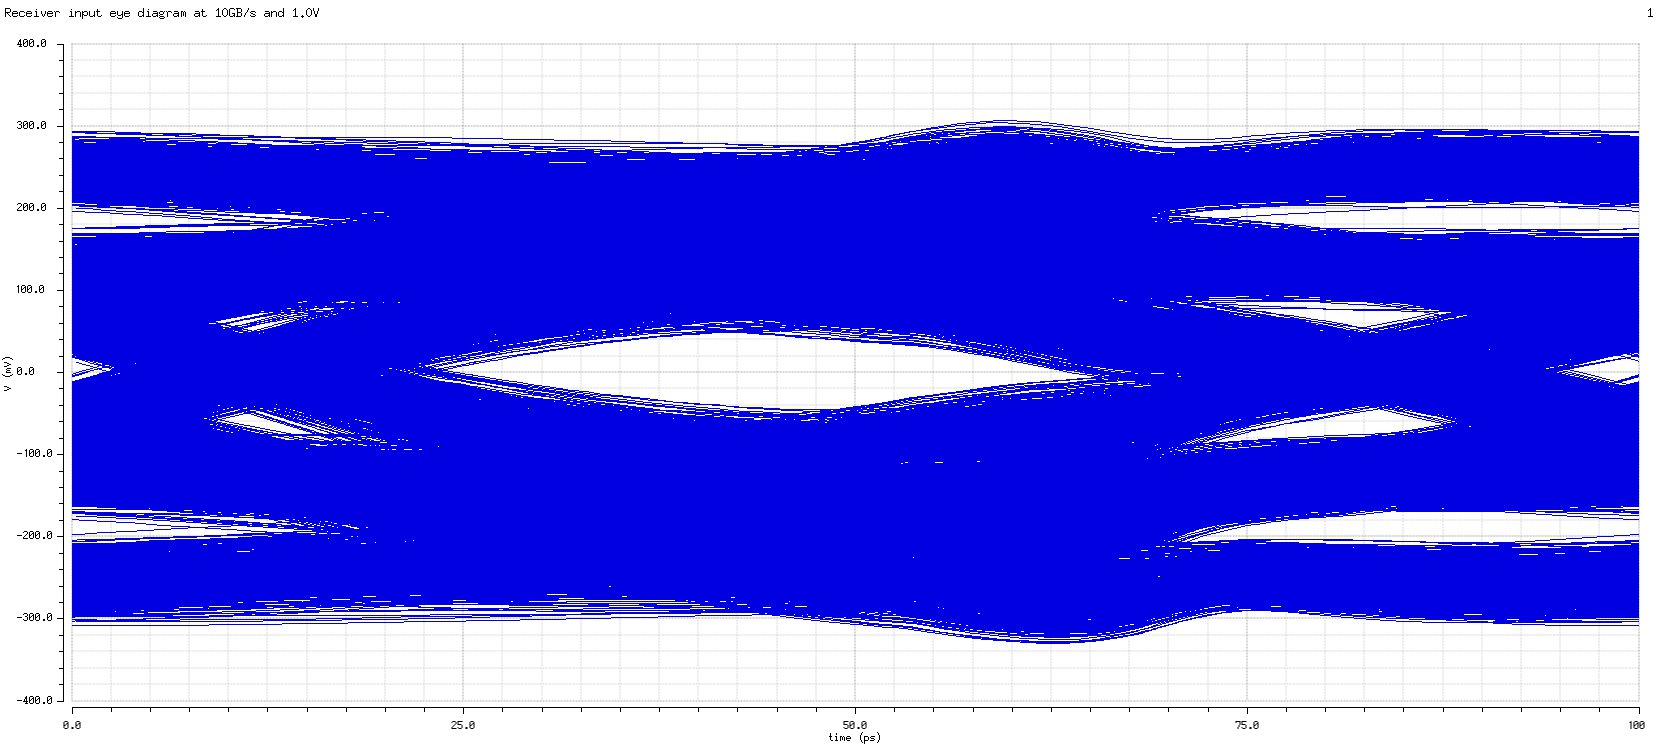
\includegraphics[scale=0.4]{img/eye_rx_10gbs_5000.jpg}}
  \subfigure[2Gb/s at 0.7V]
  {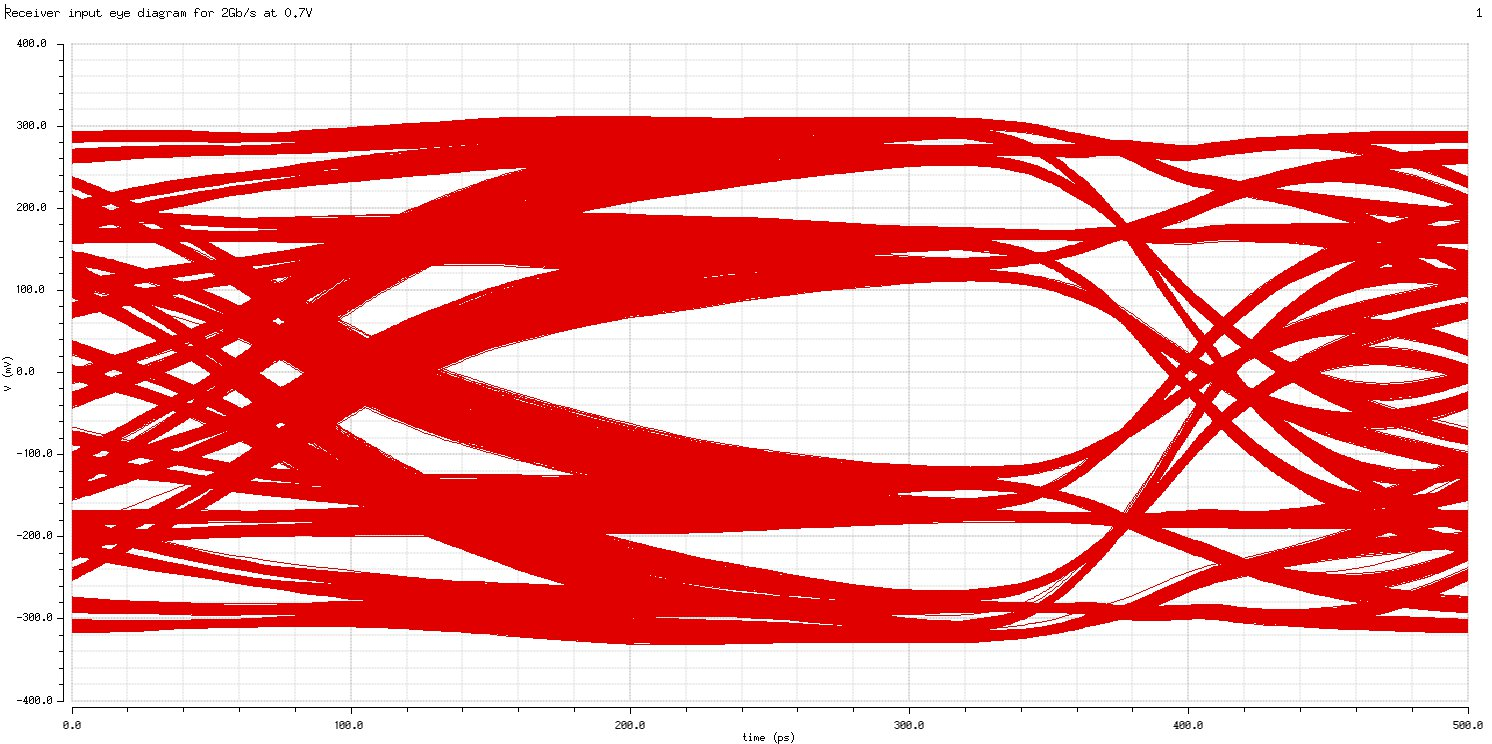
\includegraphics[scale=0.4]{img/eye_rx_2gbs_5000.jpg}}
  \caption{Eye diagram at the receiver input for \unit[5000]{UI}}
  \label{fig:rx_out_eye}
\end{figure}
\section{Performance results}

\IEEEPARstart{T}{odo} write sth here!

%TODO table with performance/specs
%\section{Performance results}

\IEEEPARstart{T}{odo} write sth here!

%TODO table with performance/specs
%\section{Performance results}

\IEEEPARstart{T}{odo} write sth here!

%TODO table with performance/specs
\section{Performance results}

\IEEEPARstart{T}{odo} write sth here!

%TODO table with performance/specs
\section{Impedance tuning}

\IEEEPARstart{T}{odo} write sth here!

%TODO tuning range graph
\subsection{Power consumption}
The power consumption at \unit[10]{Gb/s} PRBS15 data and \unit[1]{V} power supply as well as at \unit[2]{Gb/s} and \unit[0.7]{V} power supply is shown in table \ref{tab:power_consumption_rx}. The complete receiver consists of two receiver slices, each of them of VOA, strongARM and RS-FlipFlop (see section \ref{sec:rx_schematics}).

\begin{table}[H] %TODO add values for 2GB/s 0.7V
  \centering
  \begin{tabular}{l|l|l}
    component & \unit[10]{Gb/s} at \unit[1]{V} & \unit[2]{Gb/s} at \unit[0.7]{V}\\
    \hline
    complete receiver & \unit[2217]{\uW} & \unit[223]{\uW}\\
    clock buffers & \unit[1888]{\uW} & \unit[171]{\uW}\\
    receiver slice & \unit[164,67]{\uW} & \unit[25,92]{\uW}\\
    VOA & \unit[49,54]{\uW} & \unit[14,73]{\uW}\\
    strongARM & \unit[42,27]{\uW} & \unit[3,718]{\uW}\\
    RS-FlipFlop & \unit[72,86]{\uW} & \unit[7,471]{\uW}\\
  \end{tabular}
  \caption{Receiver power consumption with PRBS15 data}
  \label{tab:power_consumption_rx}
\end{table}

As it can be observed the total power consumption of the receiver is 2.217mA, which at 1V gives a power consumption of 2.217mW, resulting in a energy consumption of 2.217mJ per second. This gives that the energy per bit is 0.2217 pJ per bit, it seems like the power consumption of receiver is pretty decent and that future work, in reducing power consumption of the link, should be done on the transmitter.
\section{Performance results}

\IEEEPARstart{T}{odo} write sth here!

%TODO table with performance/specs
%\section{Performance results}

\IEEEPARstart{T}{odo} write sth here!

%TODO table with performance/specs
<<<<<<< HEAD
=======

>>>>>>> 3debf833a094be1a2bf5601a201b3bc4a838fbe5



% Can use something like this to put references on a page
% by themselves when using endfloat and the captionsoff option.
\ifCLASSOPTIONcaptionsoff
  \newpage
\fi

\newpage
\section{Bibliography}
\bibliography{biblio}{}
\bibliographystyle{plain}


\end{document}


